\begin{figure}[!htbp]
    \begin{centering}
        % \subfloat[subfloat-text]
        {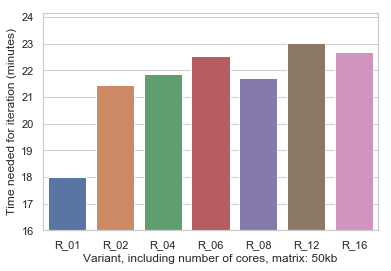
\includegraphics[scale=0.8]{figures/results/runtime_multi_50}}
        \caption[Multi-core computation time comparison]
        {\textbf{Multi-core computation time comparison} for 50kb matrix. These are
        pure computing times, excluding both pre- and post-processing. No numbers
        for ICE and KR are available. Smaller is better.}
        \label{fig:mrun50}
    \end{centering}
\end{figure}
